%\vspace{-4pt}
\subsection{Overview}
\label{sec:overview}
%\vspace{-4pt}

\begin{figure*}[t]
	\centering
		%\begin{minipage}{0.225\textwidth}
			\centering
			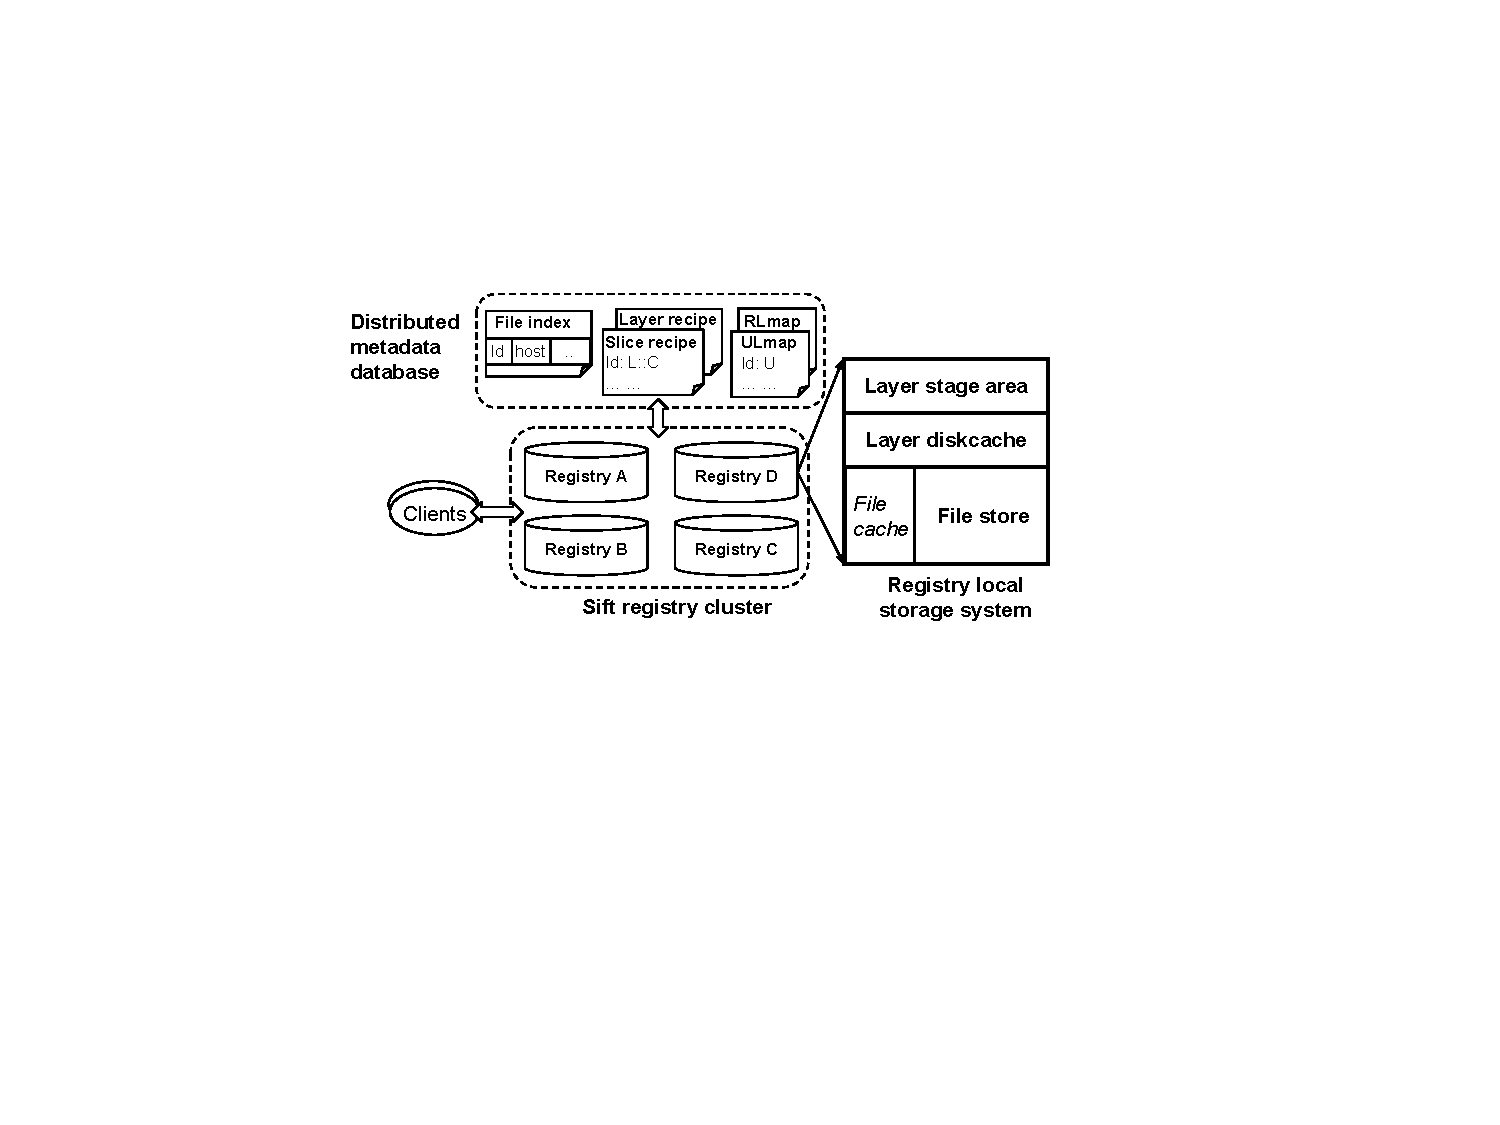
\includegraphics[width=0.9\textwidth]{graphs/sys-architecture.pdf}
%\vspace{-4pt}
			\caption{Architecture of \sysname.}
			%\label{fig:ref_count}
		%\end{minipage}
%	\begin{minipage}{0.225\textwidth}
%		\centering
%		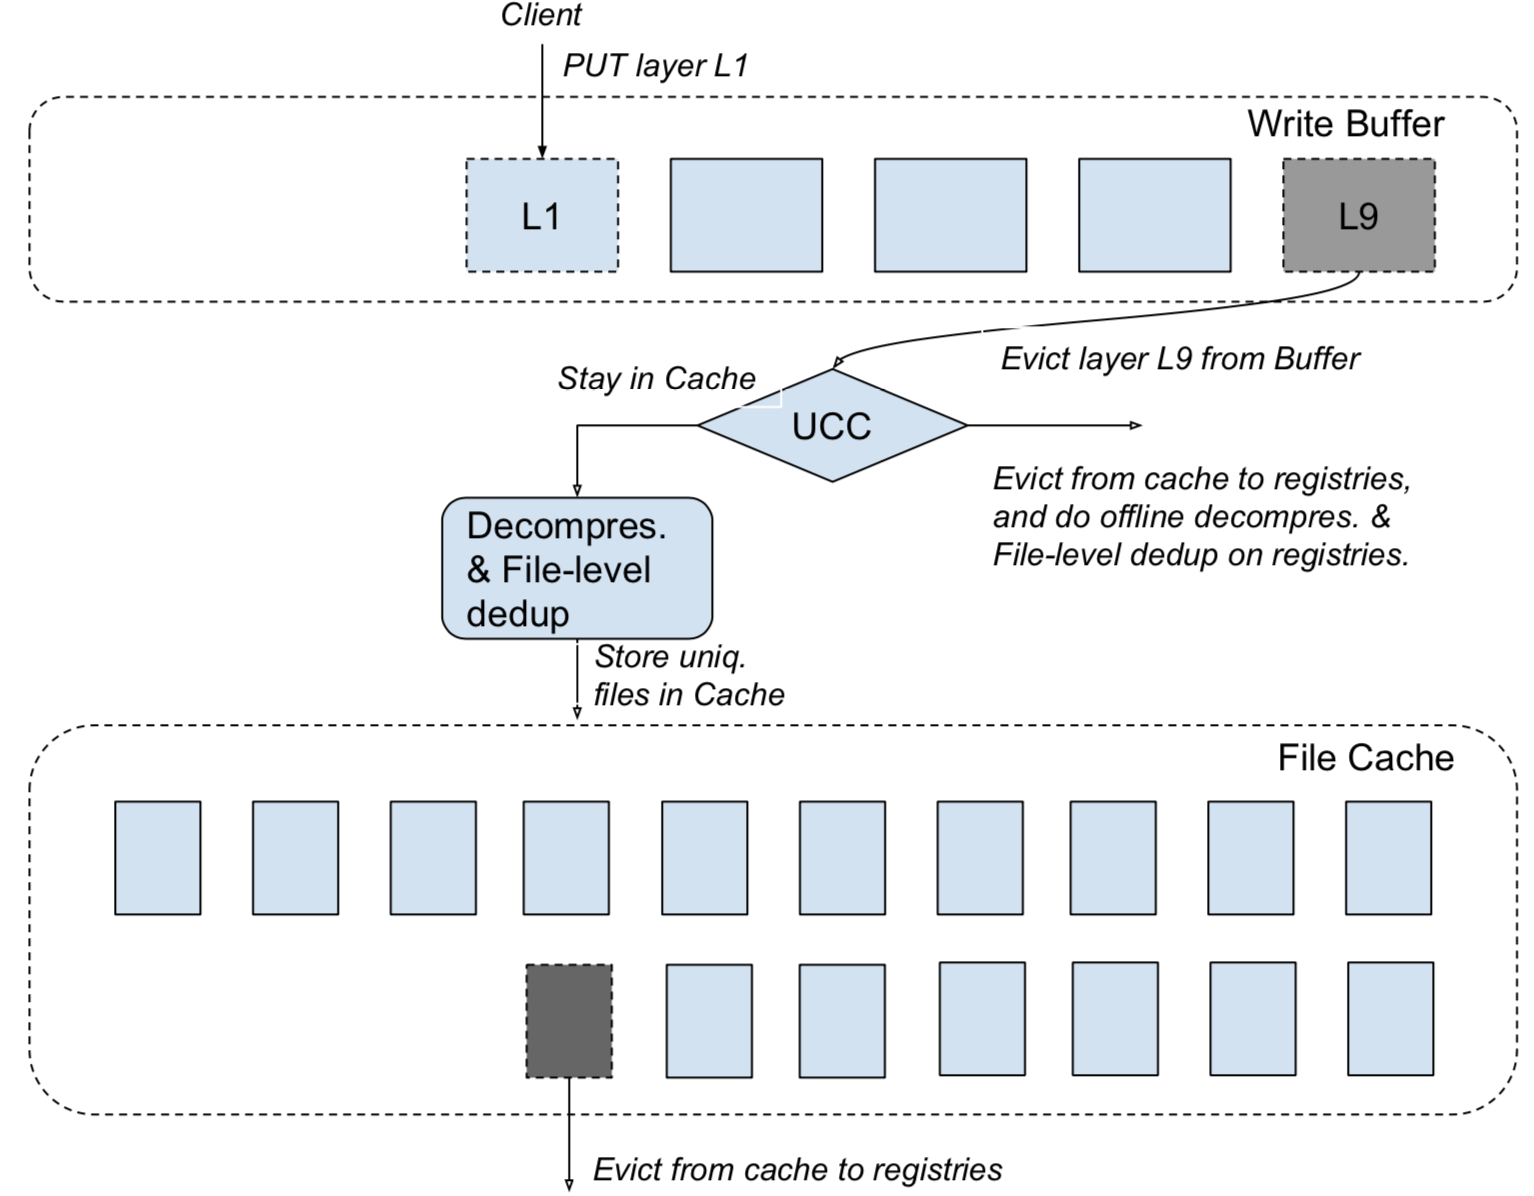
\includegraphics[width=1\textwidth]{graphs/slimmer-cache.png}
%		\caption{CDF of compress. and uncompress. layer size.}
%		\vspace{-3pt}
		\label{fig:sys-overview}
%\vspace{-4pt}
%	\end{minipage}
\end{figure*}

%\input{fig-diskcache}

%\LR{For example, here we need to first motivate, why those replication modes are there. What are the
%objectives of Sift? We want to deduplicate layers but we don't want latencies to suffer. So what is
%the problem then? Reconstructing layers is expensive. That's why we choose to have replication modes
%to trade-off storage space for performance.}
\LR{This following paragraph should be part of background. Ali, can you move it to background and fit
it in there? I think we should also split Figure~\ref{fig:sift-original} and also move the top part,
which describes the standard registry, to the background section.}

%\LR MOVE THIS TO BACKGROUND {START}
We first consider  a simple example of current registry backend storage system.
Upon a \texttt{push} layer request,
server \emph{A} stores the layer locally, such layer is denoted as \emph{primary layer replica}.
Meanwhile \emph{A} replicates the layer to the other two servers: 
\emph{B} and \emph{C} to maintain reliability as shown in Figure~\ref{fig:sift-original}. 
These replicated layers are denoted as \emph{backup layer replicas}.
 %shows a simple deduplication mode of \sysname's registry cluster compared with original registry cluster.
%In the original registry cluster upon  a \texttt{push} request, 
%registry \emph{A} stores the layer locally, such layer is denoted as \emph{primary layer replica}.
The subsequent \texttt{pull} layer requests can be served by 
any of the three layer replicas.%depending on the registry server's availability?
%\LR MOVE THIS TO BACKGROUND {FINISH}

Figure~\ref{fig:sift} shows the architecture of \sysname.
\sysname consists of a cluster of registry backend storage servers and a distributed metadata database. 
Storage servers store and serve both manifest and layer requests sent by clients. The
metadata database keeps all deduplication-related metadata, which is necessary to correctly restore
a deduplicated layer.
%
To reduce deduplication overhead, \sysname tries to minimize the time it takes to restore a layer
during a \texttt{pull} request. This is achieved by three main techniques: 1)~deduplication modes;
and 2)~parallel layer reconstruction; and 3)~predictive cache prefetching.

\paragraph{Deduplication modes}

\sysname makes use of the fact that most registries employ some form of layer replication
for fault tolerance and availability. The idea is that, instead of deduplicating every layer replica,
\sysname allows to configure, how many replicas of a layer should be deduplicated and
how many replicas should be kept in their original state for faster serving.

A \emph{basic deduplication mode} (B-mode) $n$ defines that \sysname should keep $n$ layer
replicas and deduplicate the remaining $R-n$ layer replicas, where $R$ is the
layer replication level.
%
%by deduplicating a different number of layer replicas, denoted as
%\textbf{basic deduplication modes (i.e, B-modes)}.
%
At one extreme, B-mode $R$ means that no replica should be deduplicated and hence, provides the best
performance but no data reduction. At the other end, B-mode $0$ deduplicates all layer replicas, i.e. it
provides the highest deduplication ratio but adds restoration overhead for every \texttt{pull} request.
The remaining B-modes in between allow to trade off performance and data reduction.

For heavily skewed workloads, \sysname also provides a \emph{selective deduplication mode} (S-mode). The
S-mode utilizes the skewness in layer popularity, observed in~\cite{dockerworkload}, to decide, how many
replicas should be deduplicated for each layer individually. As there are hot layers that receive the
majority of \texttt{pull} requests, S-mode sets the number of layer replicas inversely proportional to
its popularity. This means that hot layers have less deduplicated replicas and hence, can be served
faster. On the other hand, cold layers have more deduplicated replicas to improve storage utilization.
%
%and deduplicates the rest
%to provide a better performance for hot layers
%and deduplicate the cold layer.

%To exploit replication technique for good performance and deduplication technique for data reduction,
%%Similar to the original registry cluster, 
%\sysname maintains a certain number of layer replicas for layer accesses 
%while \emph{deduplicating} the rest for space savings.
%
Figure~\ref{fig:sift-original} shows an example for B-mode $1$ with $R=3$.
\sysname maintains a single layer replica (the \emph{primary layer replica}) on server A for newly 
pushed layers.
%
%first stores three layer replicas for 
%a newly \texttt{pushed} layers on three different servers: %\emph{A}, \emph{B}, and \emph{C}. 
%
The remaining two backup layer replicas %server roles/group discussed later, a forward reference maybe?
are \emph{deduplicated}, i.e. any
duplicate files are discard while \emph{unique files} are kept.
The unique files are replicated and saved on different servers B and C.
%
%\emph{A} stores the while \emph{B} and \emph{C} store
%
%Then, one of the backup layer replicas (say, at server B) is \emph{deduplicated} into unique files, denoted as 
%\emph{primary file replicas}. %
%%\HA{It is not clear in the previous sentence that primary file replica is a collection of all the unique files 
%constituting the layer or a file (one file)? Also, we should state why only one server is deduplicating i.e. 
%the performance effect}
%After that, each unique file is replicated and stored onto the remaining servers (in this case, \emph{C}),
%denoted as the \emph{backup file replicas}.
%In the end, the two backup layer replicas at \emph{B} and \emph{C} are discarded while the primary layer
%replica at \emph{A} remains.
%
Any subsequent \texttt{pull} layer requests are sent to server A since it stores a complete layer replica.
If server A crashes, server B or C is needed to rebuild the layer and serve the \texttt{pull} request.
%for the incoming \texttt{pull} layer request.
%As a result, 
%Thus, \sysname provides the same level of redundancy as the original registry backend storage cluster. 

To support the different deduplication modes, \sysname divides storage servers into two 
groups (see Figure~\ref{fig:sift}):
a \emph{primary cluster} consisting of \emph{P-servers} and a \emph{deduplication cluster}
consisting of \emph{D-servers}.
P-servers are responsible for storing full layer replicas and manifest replicas
while D-servers \emph{deduplicate} layer replicas at the file level, 
store the unique files, and replicate them.
%
%The reason we separately store layer replicas and 
%file replicas is to make sure that
The split is necessary to ensure that
layer replicas and its containing file replicas are stored on different servers to maintain
fault tolerance.

%As shown in Figure~\ref{fig:sift},
P-servers and D-servers form a two-tier storage hierarchy:
In the default case, the primary cluster serves all incoming \texttt{pull} requests.
If a request can't be served from the primary cluster, for example, due to a node failure,
it will forwarded to the deduplication cluster and the requested layer will be restored.
%
%\LR{It would be good to briefly mention here, how we split servers into P- and D-servers, or make a forward
%reference to the place, where we actually discuss it in detail.}
%
\LR{Here we also need to talk about dealing with overloaded (not just crashed) P-servers.}

\paragraph{Parallel layer reconstruction}

\sysname speeds up layer reconstruction through parallelism. As shown in Figure~\ref{fig:sift},
each D-server's local storage is divided into three parts: layer stage area, preconstruction cache,
and file store.
%
%\LR{Should it be 4 parts? Why do we not include the file cache? I think file cache should also
%be explained here.###### remove file cache from graph}

The layer stage area temporarily stores newly added layer replicas.
After \texttt{deduplicating} a replica, the resulting unique files are stored in a content 
addressable \emph{file store} and replicated to the peer servers to
provide redundancy. Once all replicas have been stored, the layer replica is deleted from the
layer stage area. 

\sysname distributes the layer's unique files
% and \emph{shared files}
onto several servers (see~\S\ref{sec:dedup-desgin}).
%such that
%a %\HA{is it a deduplicated layer replica? ##### no, layer = unique files + shared files. to rebuild a layer, we need to 
%consider shared file as well}
%
All files on a single server belonging to the same layer are called a \emph{slice}. A slice
has a corresponding \emph{slice recipe}, which defines the files that are part of this slice,
and a \emph{layer recipe} defines the slices needed to reconstruct the layer. This information
is stored in \sysname{}'s metadata database
%Deduplication related metadata such as \textbf{layer recipe} and \textbf{slice recipe}
%%, \textbf{layer index}, and \textbf{file index} 
%is kept in a \emph{distributed database} (Figure~\ref{fig:sift})
for reliability, consistency, and fast accesses. 
%The partition on each server can rebuild a \textbf{slice} of the layer. 
%
This allows D-servers to rebuild layer slices in parallel and thereby, improve reconstruction
performance.
%To rebuild a layer, the D-server first rebuilds the layers' slices in parallel 
%according to the associated \textbf{slice recipes} and \textbf{layer recipe}.
%After that D-server concatenates the slices into a layer (see section~\ref{sec:dedup-desgin}).
%
\LR{We should also explain here the File and Layer indeces shown in the Figure.}

\paragraph{Predictive cache prefetching}

To improve the layer access latency, \sysname employs a cache layer in both the
primary and the deduplication cluster.
%
Each P-server has a in-memory \emph{user-behavior based superfetch cache}
to reduce disk I/Os as detailed in~\S\ref{sec:cache-design}.
\LR{Add short explanation on how it works and introduce RLmap and ULmap.}
%as shown in Figure~\ref{fig:sift}.

Additionally, to avoid layer restoring overhead,
each D-server maintains an on-disk layer cache (called \emph{user-behavior based preconstruct cache}).
D-servers try to preconstruct likely to be accessed layers and load them into their
preconstruct cache.
\LR{Again, put short explanation of how it works using RLmap und ULmap.}

%To do that,
%D-server
%the layer's associated \textbf{layer recipe} (see section~\ref{sec:restore-design})
%
%The preconstruct cache is a write-through cache; when layers are evicted from the diskcache, they are simply discarded.
%
%Slice recipe and layer recipe are used to restore slices and rebuild layers.
%Layer index and file index records \emph{content fingerprints} that are uniquely mapped to the associated physical layers and files respectively. %psychical file based on
%Moreover, \sysname keeps track of user accesses and repository status, 
%denoted as \textbf{ULmap} and \textbf{RLmap}, 
%and stores them into the distributed metadata database.
  
%The \emph{Preconstruct cache} on a D-server is an on-disk layer cache 
%which hosts preconstructed popular layers for later layer accesses to mitigate layer restoring latency (see section~\ref{sec:cache-design}).
%As shown in Figure~\ref{fig:cache}, 
%When a P-server crashes,
%the \texttt{pull} layer request will be served from a D-server. \HA{Isn't the previous sentence already stated above?}
%%
%\LR{The following is a bit unclear. Is the stage area the same as the preconstruction cache?}
%%
%If the \texttt{pull} layer request has a hit in the D-server's layer stage area (i.e. a layer replica has not been deleted yet),
%the request will be served from layer stage area.
%\LR{Now that we also store non-deduplicated layers, we need to make sure that the preconstruction cache still
%makes sense. For example, if we have a `fully deduplicated` mode, in which we only store deduplicated layers
%(i.e. number of P-servers = 0), then the preconstruction cache would be useful.}


%In the following, we first describe different deduplication modes provided by \sysname.
%Then, we describe how \sysname performs layer deduplication and layer restoring.

%\paragraph{Deduplication modes}
\label{sec:dedup-mode}

To satisfy different space saving and performance requirements,
\sysname provides two kinds of deduplication modes:
Basic deduplication modes and selective deduplication modes, denoted as \emph{B-modes} and \emph{S-modes}.
B-mode mantains a certain amount of layer replicas for each layer and deduplicates the rest layer replicas.
While S-mode mantains a number of layer replicas for different layer proportionate to their popularity.

%\subsubsection{Basic deduplication modes}
Assume that registry storage system uses R-way replication.
Consider that layer dataset deduplication analysis~\cite{xxx} shows a file-level deduplication ratio of 2$\times$.
Thus, the average layer deduplication ratio for the layer dataset~\cite{xxx} is 2$\times$.
% subil: need clarification here. where is the 2x coming from

B-mode \emph{r} is defined as keeping \emph{r} layer replicas and deduplicating the rest of layer replicas, where $r \leq R$. 
The space saving is calculated by following equation~\ref{eq:b-savings}.
\begin{equation}\label{eq:b-savings}
Space savings = \frac{R-(r+\frac{1}{2}(R-r))}{R} = \frac{R-r}{2R}
\end{equation}

Layer pulling performance largely depends on registry server load.
Assume that the total number of P-servers and D-servers are \emph{P} and \emph{D} especially.
The total \texttt{pull} layer request load is \emph{L}.
Consequently, the average server load is $\frac{L}{P}$ and $\frac{L}{P+D}$ for \sysname and original registry respectively.
Note that original registry is \sysname's B-mode \emph{R}, which represents the best pulling layer performance with no space savings.
The performance degradation can be calculated as:
%$$
 %$\emph{f}_\frac{L}{P} \times \theta_{r}$. 
 
 \begin{equation}\label{eq:c-pull}
Performance degradation =  F(L, P, D, \delta_{R-r})
 \end{equation}
 $\delta_{R-r}$ means the performance degradation caused by load variance among different servers impacted by replication level.

%\subsubsection{Selective deduplication modes}
In S-mode, the number of layer replicas \emph{r} is proportional to their popularity ($r \leq R$).
Layer popularity is calculated as $\frac{\emph{l}_{pcnt}}{L}$, 
where $\emph{l}_{pcnt}$ is the total number of pulling request count to layer \emph{l}.  
Consequently, the number of layer replicas $r_{l}$ for layer \emph{l} is
%\emph{r} ($r \leq R$) is calculated as:
$r_{l} = R \times \Phi (\frac{\emph{l}_{pcnt}}{L})$, 
where $\Phi (\frac{\emph{l}_{pcnt}}{L})$ denotes a replication factor.

The space savings for S-mode is calculated as following equation~\ref{eq:s-savings}.
\begin{equation}\label{eq:s-savings}
Space savings = \frac{\sum\limits_{l=1}^n{R-(r_{l}+\frac{1}{2}(R-r_{l}))}}{\sum\limits_{l=1}^n{R}} 
\end{equation}
% subil: I feel like there should be a summation over the whole numerator and a summation over the whole denominatorgit 

The performance degradation is:
  \begin{equation}\label{eq:s-pull}
Performance degradation =  F(L, P, D, \delta_{R-r_{l}})
 \end{equation}
where $\delta_{R-r_{l}}$ means 
the performance degradation caused by load variance among different servers impacted by different replication levels.
 

%\sysname uses a fast and reliable distributed database to 
%%, and unique files after layer deduplication
%The metadata such as layer recipes and slice recipes which
%Each server in the \sysname~registry cluster uses part of its storage for storing assembled (\ie preconstructed) layers. 
%We name such storage: user behavior based layer preconstruct cache (\preconstructcachename).
%Another part, a layer restoring performance--aware deduplication system (\dedupname system), is for storing deduplicated files. 
%Such files' metadata (\eg Docker image manifests) is kept in a metadata store; a distributed NoSQL database for 
%reliability, consistency, and fast accesses.
%
%

%\paragraph{Push}
%
%%As shown in Figure~\ref{fig:sys-overview}, 
%Consider a Docker client, client \textit{A}, who creates a new hello-world image
%\texttt{hello-world:new}
%from the official image which only contains a single layer \textit{L1}. 
%Pushing a new version of hello-world image corresponds to performing a PUT of layer \textit{L2} to the registry and a PUT of manifest to the metadata store as shown in Figure~\ref{fig:sys-overview}. 
%%first PUT
%Because the registry already stores \textit{L1}, 
%%only the modifications to the hello-world image that are commited as a new layer \textit{L2}, 
%only the compressed \textit{L2} tarball is PUT to the registry reflecting the modifications to the hello-world image.
%When \sysname~receives \textit{L2}, 
%it will cache \textit{L2} in the \preconstructcachename~for later accesses,
%and at the same time submit \textit{L2} to the backend storage system (Figure~\ref{fig:sys-overview}).
%The \preconstructcachename~uses write through policies. 
%Since layers are immutable, no data consistency issue exists between the \preconstructcachename~and the backend storage system.
%% Second PUT (manifest)
%The addition of layer \textit{L2} to the hello-world image is reflected in the manifest \textit{M1:0} which is PUT to the registry.
%Putting the new manifest \textit{M1:0} to the registry for the new image \texttt{hello-world:new} conlcudes the process of pushing it.
%
%
%
%The \dedupname~process runs periodically to deduplicate compressed layer tarballs (detailed in~\cref{sec:dedup-desgin})
%into unique files to save storage space.
%As shown in Figure~\ref{fig:sys-overview}, cold layer \textit{L2} is selected to be deduplicated.
%The \dedupname~process decompresses \textit{L2}, removes duplicate files from the \emph{uncompressed} \textit{L2}, and  evenly distributes the remaining unique files across the registry servers.
%This way, each server stores a 
%%\textbf{deduplicated slice}
%unique \textbf{slice}
% of the deduplicated \textit{L2}, from which a layer comprising a \textbf{slice} of \textit{L2}
%can be constructed and cached in the \preconstructcachename. We define such layer as a {\em slice layer}.
%We define all the per-server files belonging to a layer as a {\em deduplicated slice}. 
%Each server stores deduplicated slices belonging to many layers. 
%A layer is represented as a set of deduplicated slices that are distributed across multiple servers.
%The layer can be restored 
%%to a compressed layer tarball 
%from those distributed slices. 
%Such distribution allows restoring a layer in parallel.
%%To do that, 
%%\dedupname~process uses copy-on-write to update the old manifest \textit{M1:0} by adding slices' digests into it 
%%and generates new manifest \textit{M1:1} as shown in Figure~\ref{fig:sys-overview}.
%To do that, the \dedupname~process generates a new manifest \textit{M1:1} that holds, in addition to the contents of the old manifest \textit{M1:0}, the digests to the unique slices %comprising
%that make up the layer as shown in Figure~\ref{fig:sys-overview}.
%The slice digest is calculated by hashing the slice content~\cite{xxx}.
%
%\paragraph{Pull}
%
%As shown in Figure~\ref{fig:sys-overview},
%when client \textit{C} pulls an official image \texttt{hello-world} from the registry,
%\sysname~first checks if the requested layer \textit{L1} is present in~\preconstructcachename.
%If so, the \texttt{GET} layer request will be served by the cache.
%Otherwise, the \dedupname~system starts a parallel layer restoring process by serving slice layers from their hosting servers.
%For example, when client \textit{B} pulls the \texttt{hello-world:new} image from the registry,
%\sysname~sends the latest manifest (\textit{M1:1}) to client \textit{B}.
%After receiving \textit{M1:1}, client \textit{B} 
%%first 
%parses \textit{M1:1} to get a list of slice digests for \textit{L2}.
%Then, instead of sending a ``\texttt{GET layer L2}'' request, client \textit{B} will send multiple ``\texttt{GET slice of L2}'' requests to the registry.
%As shown in Figure~\ref{fig:sys-overview}, client \textit{B} sends ``\texttt{GET slice S1}'', ``\texttt{GET slice S2}'', and 
%``\texttt{GET slice S3}'' to the registry 
%since \textit{L2} is comprised of the slices \textit{S1}, \textit{S2}, and \textit{S3}.
%These requests are forwarded to the servers that store the corresponding deduplicated slice of \textit{L2}.
%%On \sysname~side, \textit{L2} is stored as deduplicated slices distributed across different servers.
%The servers will start to restore slices, \ie compose slice layers, from local deduplicated slices and send the compressed slices to the client 
%in parallel %as shown in Figure~\ref{fig:sys-overview}. 
%When client \textit{B} receives all the slices, it decompresses them together into an uncompressed layer.
%
%\paragraph{Docker client modifications}
% 
%To interact with \sysname, the Docker client is modified to 
%parse \sysname~manifests that include additional attributes, %-- 
%\ie slice digests.
%Also, if slice digests are present in a layer object in the manifest JSON file, 
%the client will replace ``\texttt{GET layer}'' request with multiple ``\texttt{GET slice}'' requests.
%Moreover, when the client receives the slices from registry, 
%the client decompresses these slices together into an uncompressed layer.  





%When a user requests a
%layer that is not present in the layer buffer, the request is forwarded to the
%file cache (detailed in~\cref{sec:design_operations}). 
%If a layer is also not found in the
%file cache, the request is forwarded to the backend dedup storage system.
%Note that after layer deduplication, unique files are
%scattered across multiple servers. 
%We define all the per-server files belonging to a layer as a {\em slice}. 
%A server stores slices for many layers, and a layer is composed of slices stored on multiple servers.
%To avoid the network latency caused by fetching slices from different servers and
%assembling them into a whole compressed layer, we split a \texttt{pull} request 
%into several~\texttt{pull slice}~requests. Those requests will then be
%forwarded to all the backend servers that store the requested
%layer's slices. 
%After a~\texttt{pull slice}~request is received, each backend server compresses the slice 
%and directly sends it back to the user.
%We modify the Docker client
%interface such that when it receives all the compressed slices, it can
%decompress them into a single layer. 
%Furthermore, compressing slices in parallel considerably lowers the layer compression latency,
%since compression time depends on the size of the
%uncompressed data.
%to cache layers and cache unique files after decompression and deduplication,
%respectively.  consists of a \emph{layer buffer} and a \emph{file cache}.  The
%layer buffer stores all the newly pushed layers in memory.  Although accessing
%memory is very fast, the size of main memory is limited. 
%All the slices for a layer are fetched in parallel for performance improvement.






%\sysname~seamlessly integrates 
%%the management of 
%caching and deduplication on the
%backend storage system (\emph{backend dedup storage}) with Docker registries.
%%
%We address a set of unique challenges to enable this integration.
%%
%First, for caching layers, \texttt{pull} layer requests are difficult to
%predict because layers are accessed infrequently.
%In~\cref{sec:background},
%%\arb{???}, 
%we have observed that about half of the layers are not
%accessed again for at least $1.3$~hours. Which means that if we
%cache a layer, we may need to wait a long time before we observe a hit on that layer.  %(as discussed in~\cref{sec:background}).  
%This is mainly 
%because when a user pulls an image from the registry, the Docker daemon on the
%requesting host will only pull the layers that are not locally stored.
%%\Ali{I do not understand the following sentence.}
%%Moreover, we have to consider that a user might deploy an applications on
%%multiple machines, so it's not easy to predict when a user will access which layers. 
%%%\Ali{The above statement is incorrect. You have to distinguish between GET layer requests
%%that are issued after a (PUSH layer + GET manifest) request and a normal GET layer request.
%%FAST paper only talk about case 1. Whereas you are generalizing that any GET layer request
%%should have a precedent GET layer request which is wrong. We can make a case
%%that not all GET layers requests have a precedent PUSH layer request but we can
%%not say that it takes a few days, weeks, or even months for a user to make a pull
%%layer request after a push layer request.}
%%\NZ{I mean the first case, push beyond your trace collection time.}
%%
%
%Second, we can not deduplicate compressed layers. For deduplication, each layer
%needs to be uncompressed, and only then can undergo file-level deduplication. Similarly,
%to restore a layer, we need to fetch files from multiple servers, and only then compress
%them in to a tar file to serve a \texttt{pull} layer request. 
%%\arb{that can service the ??? request}\NZ{addressed}. 
%This whole process can incur a 
%considerable performance overhead on \texttt{pull} layer requests.
%Deduplication also slows down
%\texttt{push} layer requests because of its high demand for CPU, memory, I/O, and network resources.
%%\Ali{Explain how push layer requests are not effected?}\NZ{fixed}
%
%%\subsection{Design}
%To address these issues, we propose a new registry design. The key feature of our design is a user-access-history-based prefetch algorithm that helps mitigate the performance degradation due to the 
%backend dedup storage system (Figure~\ref{fig:sys-overview}). Based
%on layer access pattern we observed in~\cref{sec:background} and user access history information,
%\sysname precisely prefetch the layers that may be pulled shortly.
%%has not been pulled in the requested repository
%%and the prefetched 
%%In this case, we can   
%%a user's active time is predictable. 
%%Thus, we leverage users' behavior, \ie
%%when a user is most likely to be active, to drive layer evictions from the cache.
%
%
%%\begin{figure}[t]
	\centering
		%\begin{minipage}{0.225\textwidth}
			\centering
			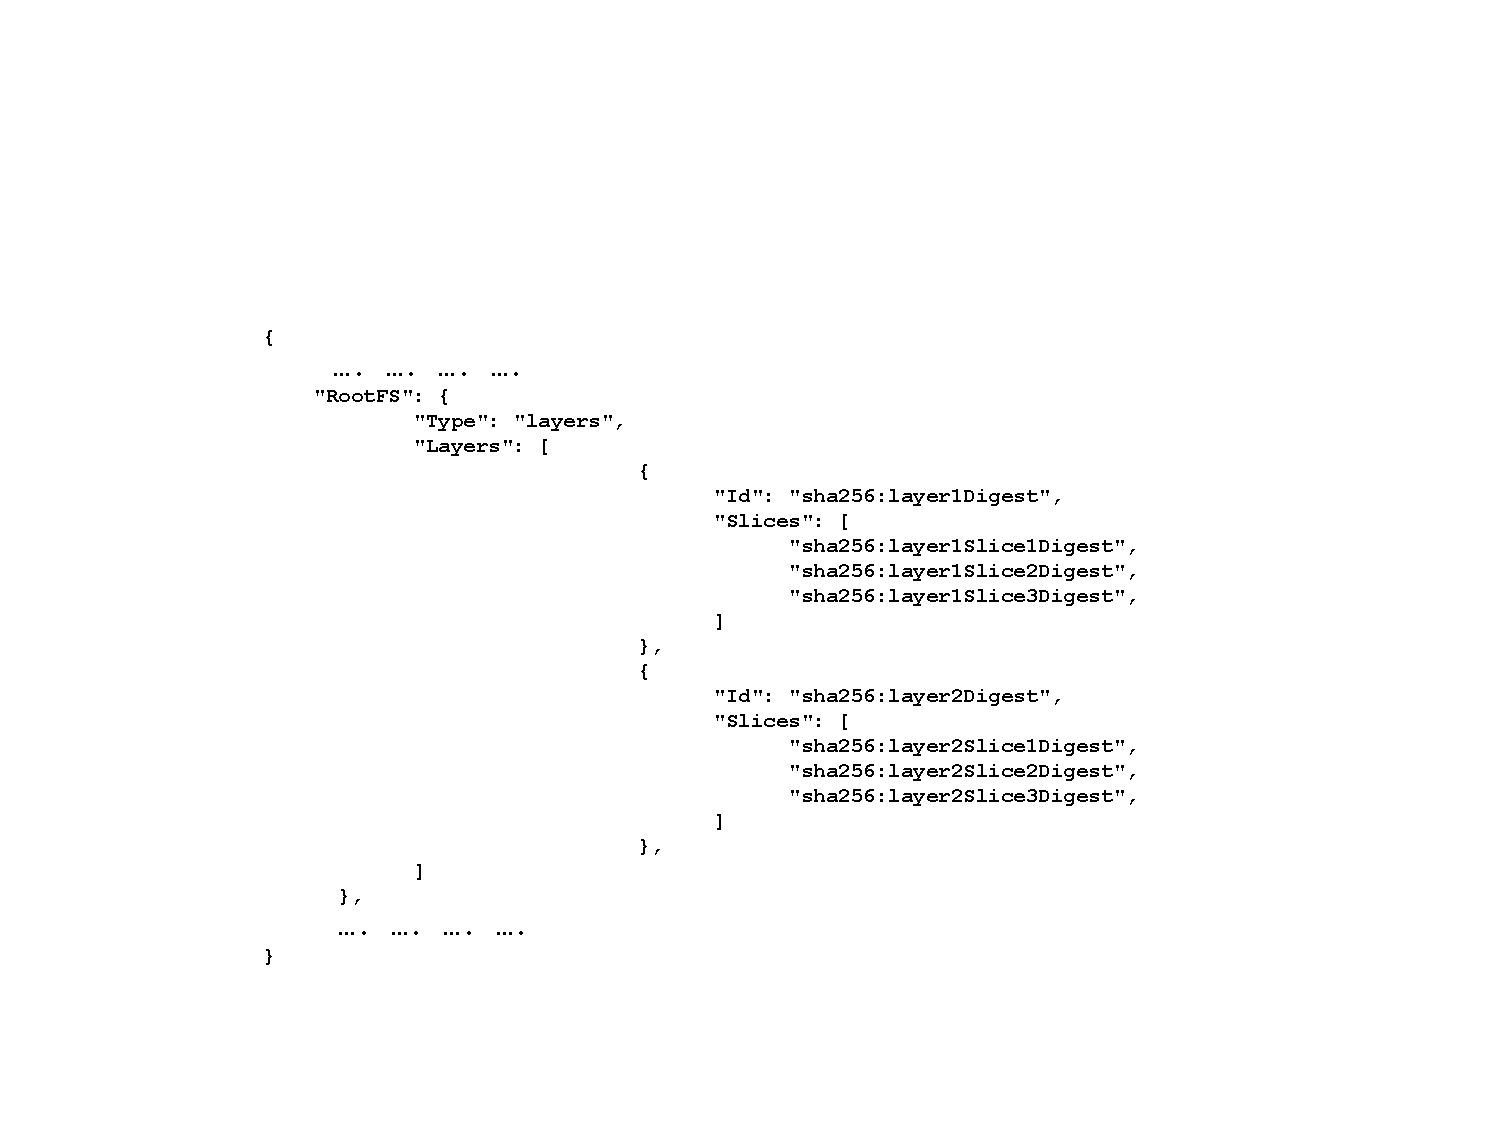
\includegraphics[width=0.4\textwidth]{graphs/fig-sift-manifest}
%\vspace{-4pt}
			\caption{\sysname~manifest.}
			%\label{fig:ref_count}
		%\end{minipage}
%	\begin{minipage}{0.225\textwidth}
%		\centering
%		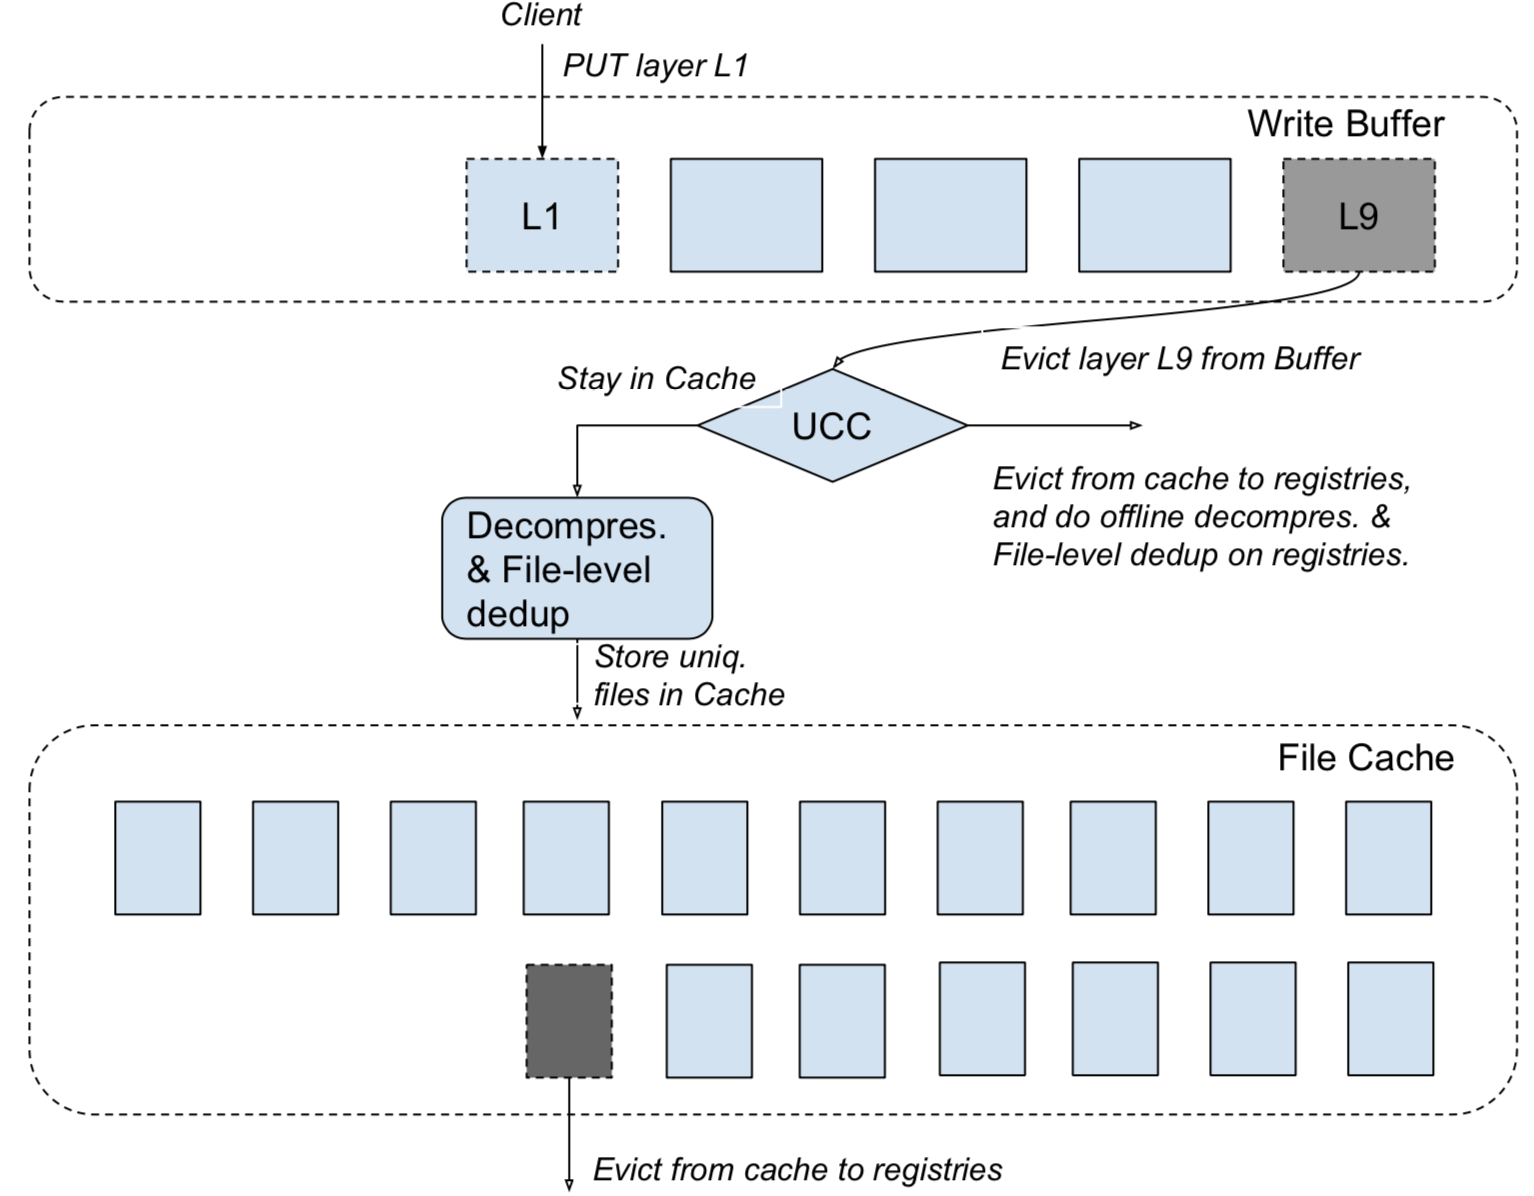
\includegraphics[width=1\textwidth]{graphs/slimmer-cache.png}
%		\caption{CDF of compress. and uncompress. layer size.}
%		\vspace{-3pt}
		\label{fig:sys-overview}
%\vspace{-4pt}
%	\end{minipage}
\end{figure}
%
%Considering that layer sizes are typically about several MB~\cite{dockerworkload}, 
%a small main memory cache will be unable to accommodate
%all prefetched layers for all active users. 
%To address this issue, we 
%create separate caches for layers and \emph{unique} files, called {\em layer buffer} and {\em file cache}, respectively. 
%%Both caches comprise both
%%main memory and flash memory.
%%Layer buffer
%%\arb{are main memory for one type and flash for the other type, or both for both types. I assumed both types of memory are used, and there are two caches. check previous sentence for correctness.}\NZ{addressed}
%Note that, layers are  compressed tarballs and buffered in layer buffer, and 
%%sent by users
% \emph{unique} files are uncompressed files from which duplicates have been removed and stored on flash-based storage. 
%%We call compressed layer cache and \emph{deduped} files cache,
%%\emph{layer buffer} and \emph{file cache}, respectively.
%For 
%cache evictions, we first evict inactive users' layers from the layer buffer.
%Next, we \emph{dedup} the evicted layers, then store the \emph{unique} files
%into the file cache (detailed in~\cref{sec:design_operations}). 
%%the following operations: decompressing each evicted layer and comparing its
%%containing files with the files that are already stored in the file cache,
%%eliminating duplicate files, that is, only storing the unique files on flash
%%storage.



 
